\documentclass{beamer}
\usepackage[utf8]{inputenc}

\usetheme{Madrid}
\usecolortheme{default}
\usepackage{amsmath,amssymb,amsfonts,amsthm}
\usepackage{txfonts}
\usepackage{tkz-euclide}
\usepackage{listings}
\usepackage{adjustbox}
\usepackage{array}
\usepackage{tabularx}
\usepackage{gvv}
\usepackage{lmodern}
\usepackage{circuitikz}
\usepackage{tikz}
\usepackage{graphicx}

\setbeamertemplate{page number in head/foot}[totalframenumber]

\usepackage{tcolorbox}
\tcbuselibrary{minted,breakable,xparse,skins}



\definecolor{bg}{gray}{0.95}
\DeclareTCBListing{mintedbox}{O{}m!O{}}{%
	breakable=true,
	listing engine=minted,
	listing only,
	minted language=#2,
	minted style=default,
	minted options={%
		linenos,
		gobble=0,
		breaklines=true,
		breakafter=,,
		fontsize=\small,
		numbersep=8pt,
		#1},
	boxsep=0pt,
	left skip=0pt,
	right skip=0pt,
	left=25pt,
	right=0pt,
	top=3pt,
	bottom=3pt,
	arc=5pt,
	leftrule=0pt,
	rightrule=0pt,
	bottomrule=2pt,
	toprule=2pt,
	colback=bg,
	colframe=orange!70,
	enhanced,
	overlay={%
		\begin{tcbclipinterior}
			\fill[orange!20!white] (frame.south west) rectangle ([xshift=20pt]frame.north west);
	\end{tcbclipinterior}},
	#3,
}
\lstset{
	language=C,
	basicstyle=\ttfamily\small,
	keywordstyle=\color{blue},
	stringstyle=\color{orange},
	commentstyle=\color{green!60!black},
	numbers=left,
	numberstyle=\tiny\color{gray},
	breaklines=true,
	showstringspaces=false,
}
%------------------------------------------------------------
%This block of code defines the information to appear in the
%Title page
\title %optional
{1.9.30}

%\subtitle{A short story}

\author % (optional)
{Nipun Dasari - EE25BTECH11042}



\begin{document}
	
		\frame{\titlepage}
	\begin{frame}{Question}
		If the distances of $\vec{P} = (x, y)$ from $\vec{A} = (5, 1)$ and $\vec{B} = (−1, 5)$ are equal, then prove
		that 3x = 2y.
	\end{frame}

	
\begin{frame}{Theoretical Solution}
	Consider the matrices A, B and P as follows:
\begin{align*}
	\vec{A} = \myvec{5 \\ 1}, \vec{B} = \myvec{-1 \\ 5}, \vec{P}= \myvec{x \\ y}
\end{align*}
The condition for distances from $\vec{B}$ to $\vec{P}$ and $\vec{A}$ to $\vec{P}$ to be equal is
\begin{align*}
	\norm{\vec{P}-\vec{A}} = \norm{\vec{P}-\vec{B}} \equiv \norm{\vec{P}-\vec{A}}^2 = \norm{\vec{P}-\vec{B}}^2
\end{align*}
Using inner products:
\begin{align*}
	\brak{\vec{P}-\vec{A}}^{T}\brak{\vec{P}-\vec{A}} = \brak{\vec{P}-\vec{B}}^{T}\brak{\vec{P}-\vec{B}}
\end{align*}
Expanding on both sides:
\begin{align*}
	\vec{P}\vec{P}^{T} - 2\vec{A}^{T}\vec{P} + \vec{A}^{T}\vec{A} = \vec{P}\vec{P}^{T} - 2\vec{B}^{T}\vec{P} + \vec{B}^{T}\vec{B}
\end{align*}
On simplification:
\begin{align*}
	\brak{-2\vec{A}^{T} + 2\vec{B}^{T}}\vec{P} = \vec{B}^{T}\vec{B} - \vec{A}^{T}\vec{A}
\end{align*} 
\end{frame}
\begin{frame}{Theoretical Solution}
LHS constant matrix:
\begin{align*}
	2\brak{\vec{B}-\vec{A}}^{T} = 2\myvec{-1-5 \\ 5-1} = \myvec{-12 & 8}	
\end{align*}
RHS constant matrix:
\begin{align*}
	\vec{B}^{T}\vec{B} - \vec{A}^{T}\vec{A} = \brak{\brak{-1}^2 + 5^2} - \brak{1^2 + 5^2} = 0
\end{align*}
From the above:
\begin{align*}
	\myvec{-12 & 8}\myvec{x \\ y} = 0 \implies -12x + 8y = 0 \implies 3x = 2y
\end{align*}
	\end{frame}
	
	\begin{frame}[fragile]
	\frametitle{C Code- equidistant check function }
	
	\begin{lstlisting}
#include <math.h>

// Returns 1 if 3x=2y within tolerance, else 0
int equidist_check(double x, double y, double tol) {
	double val = 3.0*x - 2.0*y;
	return fabs(val) <= tol ? 1 : 0;
}
	\end{lstlisting}
\end{frame}

\begin{frame}[fragile]
	\frametitle{Python Code using shared output}
	\begin{lstlisting}
		import numpy as np
		import matplotlib.pyplot as plt
		import ctypes
		import os
		
		# Load the shared library
		lib = ctypes.CDLL(os.path.abspath("./libequidist.so"))
		lib.equidist_check.argtypes = [ctypes.c_double, ctypes.c_double, ctypes.c_double]
		lib.equidist_check.restype  = ctypes.c_int
		
		def is_on_bisector(x, y, tol=1e-9):
		"""Check if point (x,y) satisfies 3x = 2y using C library"""
		return bool(lib.equidist_check(x, y, tol))
	\end{lstlisting}
\end{frame}
\begin{frame}[fragile]
	\frametitle{Python Code using shared output}
	\begin{lstlisting}		
		# Points A, B, midpoint
		A = np.array([5, 1])
		B = np.array([-1, 5])
		midpoint = (A + B) / 2
		
		# Equation: 3x=2y -> y=(3/2)x
		x_vals = np.linspace(-2, 6, 200)
		y_vals = (3/2) * x_vals
		
		# Example points to check
		points_to_check = [A, B, midpoint]
		
		# Print verification results using C library
		for p in points_to_check:
		result = is_on_bisector(p[0], p[1])
		print(f"Point {p} on bisector? {result}")
	\end{lstlisting}
\end{frame}
\begin{frame}[fragile]
	\frametitle{Python Code using shared output}
	\begin{lstlisting}
		# Plotting
		plt.figure(figsize=(6, 6))
		plt.scatter(A[0], A[1], color='red', label='A(5,1)')
		plt.scatter(B[0], B[1], color='blue', label='B(-1,5)')
		plt.scatter(midpoint[0], midpoint[1], color='black', label='Midpoint')
		
		# Perpendicular bisector line
		plt.plot(x_vals, y_vals, 'g--', label='3x = 2y (Perp. bisector)')
		
		# Mark example points
		for p in points_to_check:
		plt.scatter(p[0], p[1], label=f"Point {p}")
	\end{lstlisting}
\end{frame}
\begin{frame}[fragile]
	\frametitle{Python Code using shared output}
	\begin{lstlisting}
		# Decorations
		plt.title("Perpendicular Bisector of A and B: 3x=2y")
		plt.xlabel("x")
		plt.ylabel("y")
		plt.legend()
		plt.grid(True)
		plt.axis('equal')
		plt.show()
	\end{lstlisting}
\end{frame}

\begin{frame}{Plot by python using shared output from c}
	\begin{center}
	\begin{figure}[H]
		\centering
		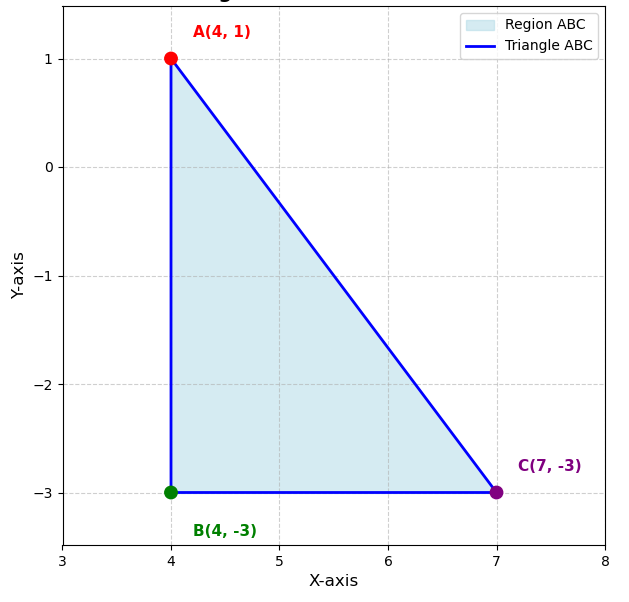
\includegraphics[width = 0.6\columnwidth]{figs/fig.png}
		\caption*{}
		\label{}
	\end{figure}
	\end{center}
\end{frame}
\begin{frame}{Plot by python only}
	\begin{center}
		\begin{figure}[H]
			\centering
			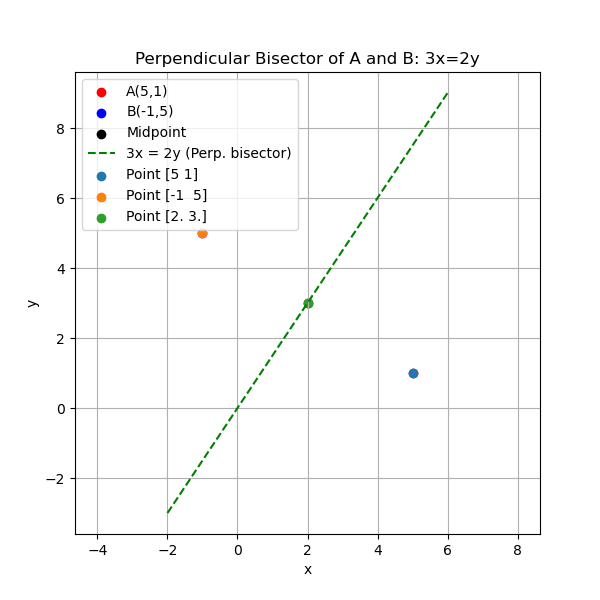
\includegraphics[width = 0.6\columnwidth]{figs/Figure_2.png}
			\caption*{}
			\label{}
		\end{figure}
	\end{center}
\end{frame}
\end{document}